% !TEX TS-program = pdflatex
% !TEX encoding = UTF-8 Unicode

% This is a simple template for a LaTeX document using the "article" class.
% See "book", "report", "letter" for other types of document.

\documentclass[11pt]{article} % use larger type; default would be 10pt

\usepackage[utf8]{inputenc} % set input encoding (not needed with XeLaTeX)

%%% Examples of Article customizations
% These packages are optional, depending whether you want the features they provide.
% See the LaTeX Companion or other references for full information.

%%% PAGE DIMENSIONS
\usepackage{geometry} % to change the page dimensions
\geometry{a4paper} % or letterpaper (US) or a5paper or....
% \geometry{margin=2in} % for example, change the margins to 2 inches all round
% \geometry{landscape} % set up the page for landscape
%   read geometry.pdf for detailed page layout information

\usepackage{graphicx} % support the \includegraphics command and options

% \usepackage[parfill]{parskip} % Activate to begin paragraphs with an empty line rather than an indent

%%% PACKAGES
\usepackage{booktabs} % for much better looking tables
\usepackage{array} % for better arrays (eg matrices) in maths
%\usepackage{paralist} % very flexible & customisable lists (eg. enumerate/itemize, etc.)
\usepackage{verbatim} % adds environment for commenting out blocks of text & for better verbatim
\usepackage{subfig} % make it possible to include more than one captioned figure/table in a single float
% These packages are all incorporated in the memoir class to one degree or another...

%%% HEADERS & FOOTERS
\usepackage{fancyhdr} % This should be set AFTER setting up the page geometry
\pagestyle{fancy} % options: empty , plain , fancy
\renewcommand{\headrulewidth}{0pt} % customise the layout...
\lhead{}\chead{}\rhead{}
\lfoot{}\cfoot{\thepage}\rfoot{}

%%% SECTION TITLE APPEARANCE
\usepackage{sectsty}
\allsectionsfont{\sffamily\mdseries\upshape} % (See the fntguide.pdf for font help)
% (This matches ConTeXt defaults)

%%% ToC (table of contents) APPEARANCE
\usepackage[nottoc,notlof,notlot]{tocbibind} % Put the bibliography in the ToC
\usepackage[titles,subfigure]{tocloft} % Alter the style of the Table of Contents
\renewcommand{\cftsecfont}{\rmfamily\mdseries\upshape}
\renewcommand{\cftsecpagefont}{\rmfamily\mdseries\upshape} % No bold!

%%% END Article customizations
\usepackage{url}
\usepackage[spanish]{babel}
\usepackage{listings} 
%%% The "real" document content comes below...

\title{BUSCAMINAS PARA ANDROID}
%\date{} % Activate to display a given date or no date (if empty),
         % otherwise the current date is printed 
         
\author{Edinson Sanchez\\Kevin Filella\\Adrian Aguilar}

\begin{document}
\maketitle

%----------------------------------------------------------------------------------------
%	TABLE OF CONTENTS
%----------------------------------------------------------------------------------------

%\setcounter{tocdepth}{1} % Uncomment this line if you don't want subsections listed in the ToC

\newpage
\tableofcontents
\newpage

\section{Introducción}
Buscaminas es un popular video juego, el cual lo podemos descargar y jugar en practicamente todas las plataformas que existen.
El objetivo del juego es limpiar un campo abstracto sin detonar las minas. Normalmente el campo se representa como una matriz cuadrada, aunque debido a la popularidad del juego se han desarrollado
muchisimas variantes en el diseño original del juego.
Imagenes tomadas de wikipedia
diseño en cubo tridimensional y diseño con muhcas minas por posicion

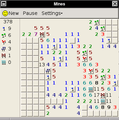
\includegraphics[height=5cm]{imagenes/119px-Firefox_Multiple_mines.png}
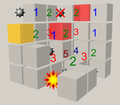
\includegraphics[height=5cm]{imagenes/120px-Cube_Minesweeper_3D.png}
%\includegraphics[height=5cm]{imagenes/File-Xbomb_triangles.png}
\subsection{Objetivo}
Nuestro objetivo en este proyecto es realizar una fiel implementacion del popular juego Buscaminas para sistemas Operativos Android.
Sabemos tambien que la competencia en el mercado es amplia por lo cual debemos , ademas de implementar fielmente las funcionalidades del buscaminas de windows, darle un toque personal y diferente  la presentacion del juego

\section{Desarrollo}
\subsection{Desarrollo inicial}
Inicialmente debido  a la naturaleza del proyecto y a las caracteristicas del curso presente tuvimos que aprender a instalar y manejar las herraminetas de desarrollo adecuadas. Ademas de aprender desde 0 a programar en Android. Con la ventaja de que su entorno de desarrollo default ofrece una IDE mastante amigable al usuario y su lenguaje de programacion es parecido al Java. 


\includegraphics[height=5cm]{imagenes/Android_robot.png}
\section{PROBLEMAS }

Durante el desarrollo de la aplicacion surgieron un sinnumero de problemas que enfrentamos para lograr construir una aplicacion estable y que cumpla con las epecificaciones del juego Buscaminas
A continuacion esta un breve resumen de los problemas mas importante que nos topamos durante el desarrollo  y lo que hicimos para solucionarlo.
Los problemas se encuentran en orden cronologico, por lo cual tambien sirven para dar una idea del progreso relativo del proyecto a traves del tiempo.

\subsection{primer problema}
\begin{center}
Vista de la aplicacion en el dispositivo Android. 

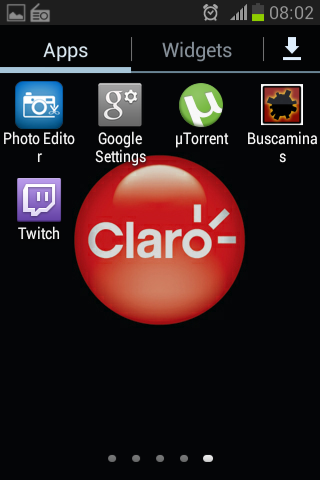
\includegraphics[width=8cm]{imagenes/Screenshot_2013-12-11-08-02-11.png}
\end{center}

Durante los primeros pasos en el desarrollo de la aplicacion no tuvimos inconvenientes reales. El parecido con el lenguaje de java hizo que facilemente implementasemos los menus y las pantallas de presentacion
Lo mas dificil de la presentacion y que nos tuvo discutiendo hasta el final fue que clase de botones o celdas utilizariamos para el buscaminas. Button, ToogleButton, ImageButton etc...

\begin{center}
Vista del Menu Principal

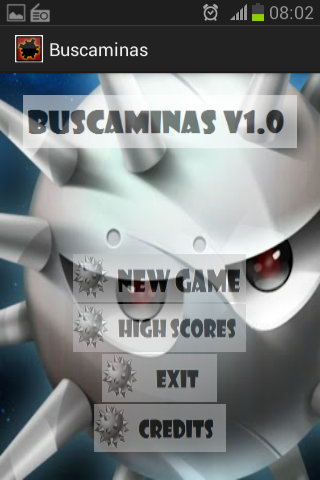
\includegraphics[width=8cm]{imagenes/Screenshot_2013-12-11-08-02-16.png}
\end{center}

\subsection{segundo problema}

La colocacion de minas y de numeros en la matriz del juego fue bastante trivial. Sin embargo empezarona  surgir problemas en los bordes de la matriz, especialmente en lo que respecta al conteo de las minas.
Al parecer nuestro algoritmo de conteo no tenia la suficiente validacion como para operar en las celdas limite de la matriz. El contador simplemente se detenia cada vez que el amgoritmo se topaba con una mina del borde, Y por las caracteristicas recursivas del mismo era bastante poco eficiente poner condiciones limites para los cuatro bordes de la matriz. Al final el problema fue solucionado enviando la funcion recursiva a cada una de las 8 celdas adyacentes individualmente a travez de bloques IF, los cuales salian cuando la celda estaba fuera de limites.


\begin{center}
Vista del la matriz del juego con todos sus elementos. 

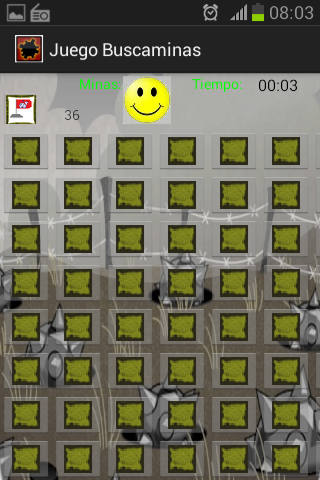
\includegraphics[width=8cm]{imagenes/Screenshot_2013-12-11-08-03-01.png}
\end{center}

\subsection{tercer problema }

Al colocar las minas trivial y aleatoriamente sobre la matriz del juego todo parecia funcionar muy bien, no fue sino luego de extensa experimentacion que hallamos un problema.
Las minas siempre se colocaban de igual o menor numero del que nosotros le enviabamos como parametro. Al principio pensamos que la causa de este problema era logica mal implementada en el contador. Luego de verificar que todo estaba aparentemente bien decidimos que la validacion no estaba funcionando y que varias minas podrian asignarse en una misma posicion, lo cual realmente era el caso ya que cuando cambiamos el metodo de validacion el problema se soluciono


\subsection{cuarto problema }

La implementacion del algoritmo recursivo para descubrir minas adyacentes vacias o numeros parecia a primera instancia facil de implementar. Pero realmente no fue asi. El algoritmo fallaba en los bordes, pero solo en el borde derecho y en el borde inferior. 
Ademas debido a la maturaleza expansiva y recursiva del mismo este se volvia perceptiblemente mas lento a medida que aumentaba el tamaño del tablero del juego. Esto debido a que la cantidad de veces que este debia ejecutarse aumenta exponencialmente 
a medida que aumentan las dimensiones de la matriz. Ademas de eso el algoritmo tambien tenia problemas cuando este llegaba al borde de la matriz de juego. Poco a poco se fueron solucionando los problemas. Uno por uno. Primero introducimos nuevas validaciones para evitar los bordes, Luego optimizamos un poco el codigo para que se ejecute mas rapido el algoritmo.

Un aspecto persistente de este problema fueron los bordes derecho e inferior. Lo solucionamos temporalmente aplicando una estricta validacion en la ejecucion del algoritmo.
Problemas con los bordes derecho e inferior del tablero se presentaron en practicamente todo el proceso de desarrollo de la aplicacion. Al final nos dimos cuenta que los limites estaban mal establecidos en la creacion de la matriz y ademas los ejes estaban intercambiados. Aunque igual pudimos lograr que el juego se ejecute normalmente a pesar de tener todos estos problemas, nos vimos obligados a reescribir codigo para arreglar el inconveniente luego del cual acabaron nuestros problemas con los bordes antes mencionados.

Luego de esto el juego podia ejecutarse con un 100% de funcionalidad.


\begin{center}
Algoritmo descubrir celdas

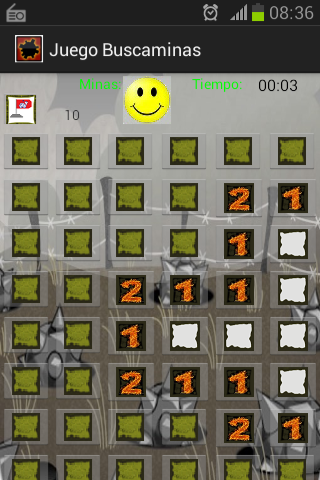
\includegraphics[width=8cm]{imagenes/Screenshot_2013-12-11-08-36-13.png}
\end{center}



\subsection{quinto problema }

Luego de solucionar bastantes problemas evidentes y que el juego se pudiese implementar de manera confiable en los niveles Facil, Intemedio y Dificil. Solo quedaba implementar el modo personalizado, en el cual el usuario decide las dimensiones de la matriz y el numero de minas que esta posee. Aqui nos dimos cuenta de algunos problemas que habian escapado nuestra atencion, como por ejemplo la incapacidad de nuestro codigo para trabajar con matrices no cuadradas. O la gigantesca cantidad de memoria que ocupaba la ejecucion del programa cuando se seleccionaba un tablero relativamente grande con pocas minas, ya que las minas y los bordes son lo unico que paran la ejecucion de la funcion recursiva. 

Estos problemas los solucionando revisando de nuevo el codigo e introduciendo nuevos elementos de validacion en algunas funciones. 
En el caso del problema de la matriz cuadrada se soluciono satisfactoriamente.
El caso de la recursividad ocupando exesiva memoria solo lo pudimos solucionar parcialemnte. 
Nos vimos obligados a implementar limites en cuanto al numero minimo de minas que el usuario puede implementar, de acuerdo a las dimensiones elegidas por el usuario.

\begin{center}
interface Personalizado. Incluye actualizacion en tiempo real del limite de minas 

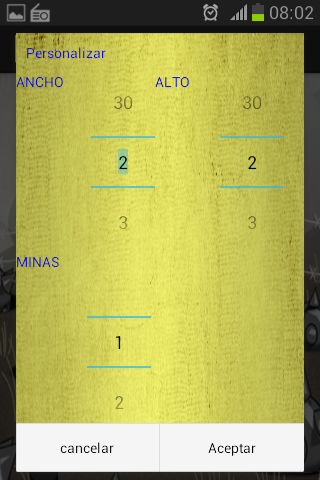
\includegraphics[width=8cm]{imagenes/Screenshot_2013-12-11-08-02-34.png}
\end{center}


\subsection{sexto problema DRAG AND DROP }

Como especificacion de este proyecto se encuentra la caracteristica de poder agregar banderas a las celdas mediante el uso de la funcionalidad Drag and Drop.
Luego de varios intentos decidimos implementar las banderas usando el metodo LongClick. el cual es compatible con anteriores versiones de Android y es mas facil de implementar.



\begin{center}
interface Personalizado. Incluye actualizacion en tiempo real del limite de minas 

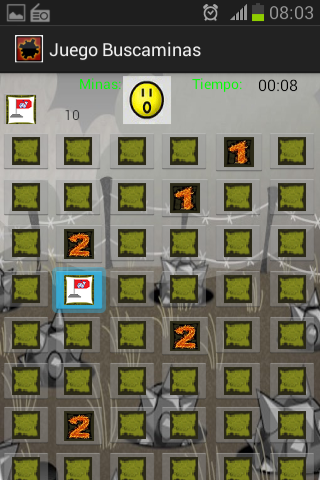
\includegraphics[width=8cm]{imagenes/Screenshot_2013-12-11-08-03-31.png}
\end{center}



\section{Alcance}

Este proyecto al momento de finalizar este documento posee toda al funcionalidad que se espera de un juego de Buscaminas. Se podria mejorar en la parte estetica y tal vez en el aspecto de facilidad de uso . 
Debido a el limite de tiempo el scoreboard del juego no esta en orden. Aunque probablemente lo este antes de finalizar la semana. Tenemos aun la limitacion en cuanto al numero de minas en la matriz personalizada, pero a pesar de todo 
podria decirse que el juego esta listo para ser probado por usuarios fuera del circulo de desarrolladores.
Ademas tambien hace falta generar el tablero automaticamente luego del primer click

\begin{center}
Pantalla de Victoria

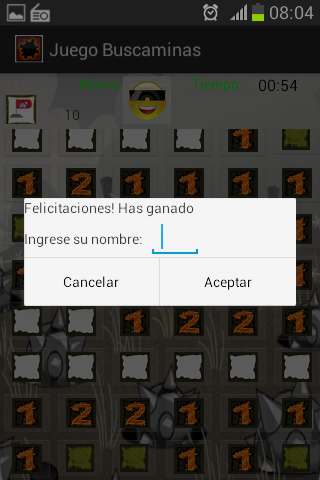
\includegraphics[width=8cm]{imagenes/Screenshot_2013-12-11-08-04-22.png}
\end{center}

\begin{center}
Ingresa el nombre del ganador


\section{Conclusion}

Como conclusion final a este proyecto de desarrollo, hay dos aspectos que deben ser resaltados, el primero es la medida en la que se ha logrado el objetivo principal, el cual es desarrollar una aplicacion de Buscaminas para Android. 
El segundo aspecto de esta conclusion tiene que ver con el resultado final, como se compara nuestra aplicacion con el Buscaminas de Windows que utilizamos como modelo. 

Sobre el desarrollo de la aplicacion , los objetivos principales fueron alcanzados satisfactoriamente. Se logro desarrollar una implementacion del juego Buscaminas para Android. 
A pesar de esto el juego tiene sus deficiencias pequeñas las cuales no pudieron ser corregidas principalmente por falta de tiempo. Como la scoreboard desordenada y el limite minimo de minas en el tablero.
Pero la aplicacion es 100% funcional en lo que a jugar Buscaminas se refiere.

Luego de un extensivo periodo de experimentacion y prueba podemos decir que el juego es divertido y funcional. 
Aunque debido a las caracteristicas de los dispositivos Android la implementacion es limitada con respecto a su contraparte de PC.
La pantalla tactil no es el metodo mas efectivo para intorducir imputs en un buscaminas. El mouse ofrece mucha mas rapidez y precision en lo que respecta a imput del juego.
Ademas el tamaño de la pantalla de los dispositivos android hace que no todo el tablero pueda ser mostrado en la pantalla, lo cual hace que jugar Buscaminas sea un poco mas complicado y tedioso
Otro aspecto es la dificultad innata para colocar na bandera en una celda, ya sea por drag and drop o LongClick, toma demasiado tiempo para ser competitivo con respecto a la version de la computadora. Es decir que un profesional de Buscaminas no puede usar nuestra aplicacion para mejorar su tiempo o su tecnica.

A pesar de que el objetivo es realizar una fiel y estable copia del Buscaminas de windows. Nos dimos cuenta que en el App Store ya existen bastantes versiones de buscaminas para Android. Por lo que decidimos darle un estilo visual direrente a nuestra implementacion para asi diferenciarnos de las demas aplicaciones en el mercado. Nos decidimos por un estilo mas natural, con un tema de la jungla y un tablero verde. Lo cual si bien es diferente al clasico ambiente sofisticado del buscaminas de windows, a manera personal nos parece agradable. Aunque para estar seguros habria que ponerlo en el mercado y juzgar dependiendo de los comentarios de los usuarios.




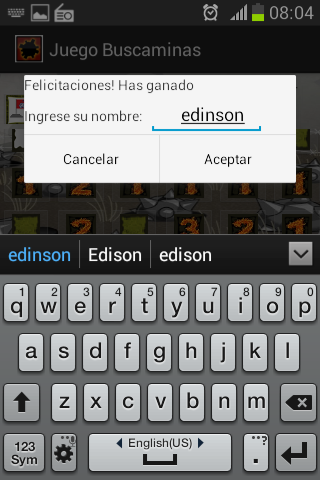
\includegraphics[width=8cm]{imagenes/Screenshot_2013-12-11-08-04-40.png}
\end{center}


\begin{center}
Scoreboard

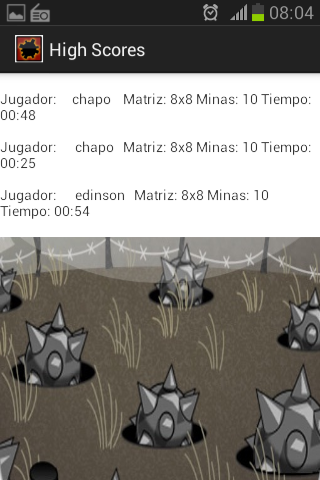
\includegraphics[width=8cm]{imagenes/Screenshot_2013-12-11-08-04-54.png}
\end{center}













  


\end{document}